\documentclass[aspectratio=169, 11pt]{beamer}

% --- Packages ---
\usepackage{graphicx}
\usepackage{tikz}
\usetikzlibrary{decorations.pathmorphing, calc, positioning, shapes.geometric, arrows.meta}

% --- Theme and Visual Settings ---
\usetheme{Madrid}
\usecolortheme{whale}

% Custom Color Palette (Steins;Gate Inspired)
\definecolor{KurisuRed}{HTML}{8D372E}     % Iconic hair color
\definecolor{LabDeepBlue}{HTML}{1A2B4C}   % Cyber/sci-fi deep blue
\definecolor{LabLightGray}{HTML}{F4F5F7}  % Clean content background
\definecolor{CRTGreen}{HTML}{39FF14}      % Terminal / divergence meter green

% Apply Custom Colors to Beamer Elements
\setbeamercolor{palette primary}{bg=KurisuRed, fg=white}
\setbeamercolor{palette secondary}{bg=LabDeepBlue, fg=white}
\setbeamercolor{palette tertiary}{bg=LabDeepBlue, fg=white}
\setbeamercolor{structure}{fg=KurisuRed}
\setbeamercolor{block title}{bg=LabDeepBlue, fg=white}
\setbeamercolor{block body}{bg=LabLightGray, fg=black}
\setbeamerfont{footnote}{size=\tiny}
\setbeamertemplate{itemize item}{\textcolor{KurisuRed}{\textbullet}}
\setbeamertemplate{itemize subitem}{\textcolor{LabDeepBlue}{\textendash}}

% Consistent spacing helpers, used instead of dashes for attributions etc.
\newcommand{\divergence}{1.048596\%}
\newcommand{\quoteattrib}[1]{{\small\color{LabDeepBlue!80} (#1)}}

% --- Presentation Metadata ---
\title[Lab Member 004]{Operation Belldandy: Project Christina}
\subtitle{Celebrating the Birthday of the Genius Neuroscientist}
\author[Cubeacon]{Future Gadget Laboratory}
\institute[FGL]{Akihabara, Tokyo}
\date{July 25, 2026}

\begin{document}

% --- Slide 1: Title Slide ---
{
\setbeamercolor{background canvas}{bg=LabLightGray}
\begin{frame}
    \titlepage
    \begin{tikzpicture}[remember picture, overlay]
        \node[anchor=south east, xshift=-0.6cm, yshift=0.5cm] at (current page.south east)
            {\tiny\color{LabDeepBlue!60} El Psy Kongroo};
    \end{tikzpicture}
\end{frame}
}

% --- Slide 2: Main Birthday Slide (Two-Column Layout) ---
\begin{frame}{Happy Birthday, Makise Kurisu!}
    \begin{columns}[c] % Vertically center aligned columns

        % Left Column: Text Data
        \begin{column}{0.55\textwidth}
            \begin{block}{Subject Profile: Lab Member 004}
                \begin{itemize}
                    \item \textbf{Name:} Makise Kurisu, aka \textit{``Christina''} (she did not choose that nickname)
                    \item \textbf{Date of Birth:} July 25, 1992
                    \item \textbf{Milestone:} Turning 34 today, a fact she would rather you not make a fuss about
                    \item \textbf{Specialty:} Neuroscience \& Theoretical Physics
                    \item \textbf{Affiliation:} Viktor Chondria University; Future Gadget Lab
                \end{itemize}
            \end{block}

            \vspace{0.3cm}

            \begin{exampleblock}{The Science of the World Lines}
                \small
                \textit{``People's feelings are memories that transcend time.''}\\[2pt]
                \raggedleft\quoteattrib{Kurisu Makise}
            \end{exampleblock}
        \end{column}

        % Right Column: The Image (1080x1439 Portrait Aspect Ratio)
        \begin{column}{0.40\textwidth}
            \begin{center}
                % The aspectratio=169 gives us plenty of horizontal room,
                % so we scale the portrait image perfectly by its height
                % to prevent it from clipping the slide headers/footers.
                
\includegraphics[height=0.75\textheight, keepaspectratio]{graphics/kurisu_birthday.png}
            \end{center}
        \end{column}

    \end{columns}
\end{frame}

% --- Slide 3: Extended Dossier ---
\begin{frame}{Lab Log: Extended Dossier}
    \begin{columns}[t]
        \begin{column}{0.5\textwidth}
            \begin{block}{Academic Record}
                \begin{itemize}
                    \item Graduated university at age \textbf{17}. A bona fide prodigy, and she will remind you of this if asked twice
                    \item Researcher at the \textbf{Brain Science Institute}
                    \item Presented a controversial time-travel paper at a Radio-Kaikan conference in Akihabara. This is the encounter that dragged her into the Lab in the first place
                    \item Later publishes memory-transfer research quietly informed by her own experience with time travel
                \end{itemize}
            \end{block}
        \end{column}
        \begin{column}{0.5\textwidth}
            \begin{block}{Lab Nicknames (courtesy of Okabe)}
                \begin{itemize}
                    \small
                    \item ``Christina'' / ``Assistant''
                    \item ``Cold-Blooded Perverted Girl Genius''
                    \item ``Mongolian Spot''
                    \item ``Celeb Seventeen'' (later ``Celeb Thirty'')
                    \item ``@Channeler''
                \end{itemize}
            \end{block}
            \vspace{0.3cm}
            \begin{alertblock}{Tsundere Alert}
                \small ``I am \emph{not} a tsundere.'' \quoteattrib{her, immediately proving the point}
            \end{alertblock}
        \end{column}
    \end{columns}
\end{frame}

% --- Slide 4: World Line Divergence Meter ---
\begin{frame}{Divergence Meter: Tracking the World Lines}
    \begin{columns}[c]
        \begin{column}{0.55\textwidth}
            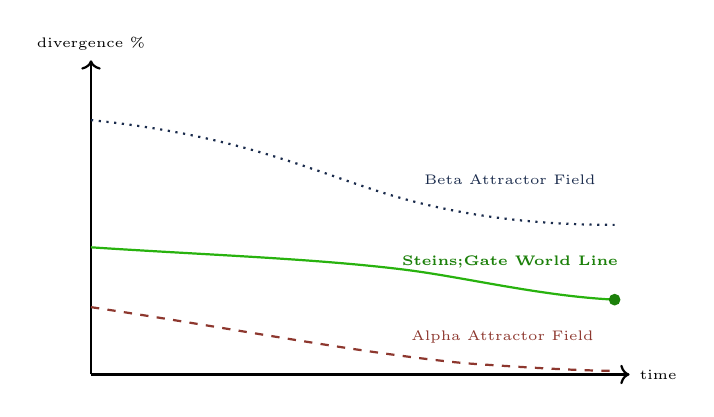
\begin{tikzpicture}[scale=0.95]
                % Axis
                \draw[->, thick] (0,0) -- (7.2,0) node[right, font=\tiny] {time};
                \draw[->, thick] (0,0) -- (0,4.2) node[above, font=\tiny] {divergence \%};

                % Beta attractor field line (middle, dotted blue)
                \draw[LabDeepBlue, thick, dotted] (0,3.4) .. controls (2,3.2) and (3,2.7) .. (4,2.4)
                    .. controls (5,2.1) and (6,2.0) .. (7,2.0);
                \node[LabDeepBlue, font=\tiny] at (5.6,2.6) {Beta Attractor Field};

                % Steins Gate world line (lower, solid green, converging)
                \draw[CRTGreen!70!black, thick] (0,1.7) .. controls (1.5,1.6) and (3,1.55) .. (4.2,1.4)
                    .. controls (5,1.3) and (6,1.05) .. (7,1.0);
                \node[CRTGreen!50!black, font=\tiny\bfseries] at (5.6,1.5) {Steins;Gate World Line};

                % Alpha attractor field line (upper, dashed red)
                \draw[KurisuRed, thick, dashed] (0,0.9) .. controls (2,0.6) and (3.5,0.3) .. (5,0.15)
                    .. controls (6,0.08) and (6.6,0.05) .. (7,0.048596);
                \node[KurisuRed, font=\tiny] at (5.5,0.5) {Alpha Attractor Field};

                % Marker at the reading
                \filldraw[CRTGreen!50!black] (7,1.0) circle (2pt);
            \end{tikzpicture}
        \end{column}
        \begin{column}{0.45\textwidth}
            \begin{block}{Reading}
                \centering
                {\Huge\ttfamily\color{CRTGreen!40!black} \divergence}\\[6pt]
                \small Divergence number of the Steins;Gate world line: the reading on which Kurisu Makise lives to see another birthday, and the one this presentation is transmitted from.
            \end{block}
        \end{column}
    \end{columns}
\end{frame}

% --- Slide 5: Full Character Reference ---
\begin{frame}{Field Reference: Standard Appearance}
    \begin{columns}[c]
        \begin{column}{0.32\textwidth}
            \begin{center}
                \includegraphics[height=0.8\textheight, keepaspectratio]{graphics/kurisu_full_profile.png}
            \end{center}
        \end{column}
        \begin{column}{0.68\textwidth}
            \begin{block}{Physical Notes}
                \begin{itemize}
                    \item Long, straight hair in chestnut-to-auburn shades, usually worn loose
                    \item Violet eyes, and a default expression best filed as ``unimpressed genius''
                    \item Signature outfit: white blouse, red tie, and a tan trench coat worn like a cape rather than a coat
                    \item Black shorts, thigh-high stockings, and boots complete the look, all quite practical for someone who spends a surprising amount of time running from the Organization
                \end{itemize}
            \end{block}
            \begin{alertblock}{Lab Safety Note}
                \small The trench coat is not lab-issued PPE. She wears it anyway, and would very much like you to stop staring.
            \end{alertblock}
        \end{column}
    \end{columns}
\end{frame}

% --- Slide 6: Lab Photo ---
\begin{frame}{Lab Photograph: Recovered from Another World Line}
    \begin{columns}[c]
        \begin{column}{0.55\textwidth}
            \begin{center}
                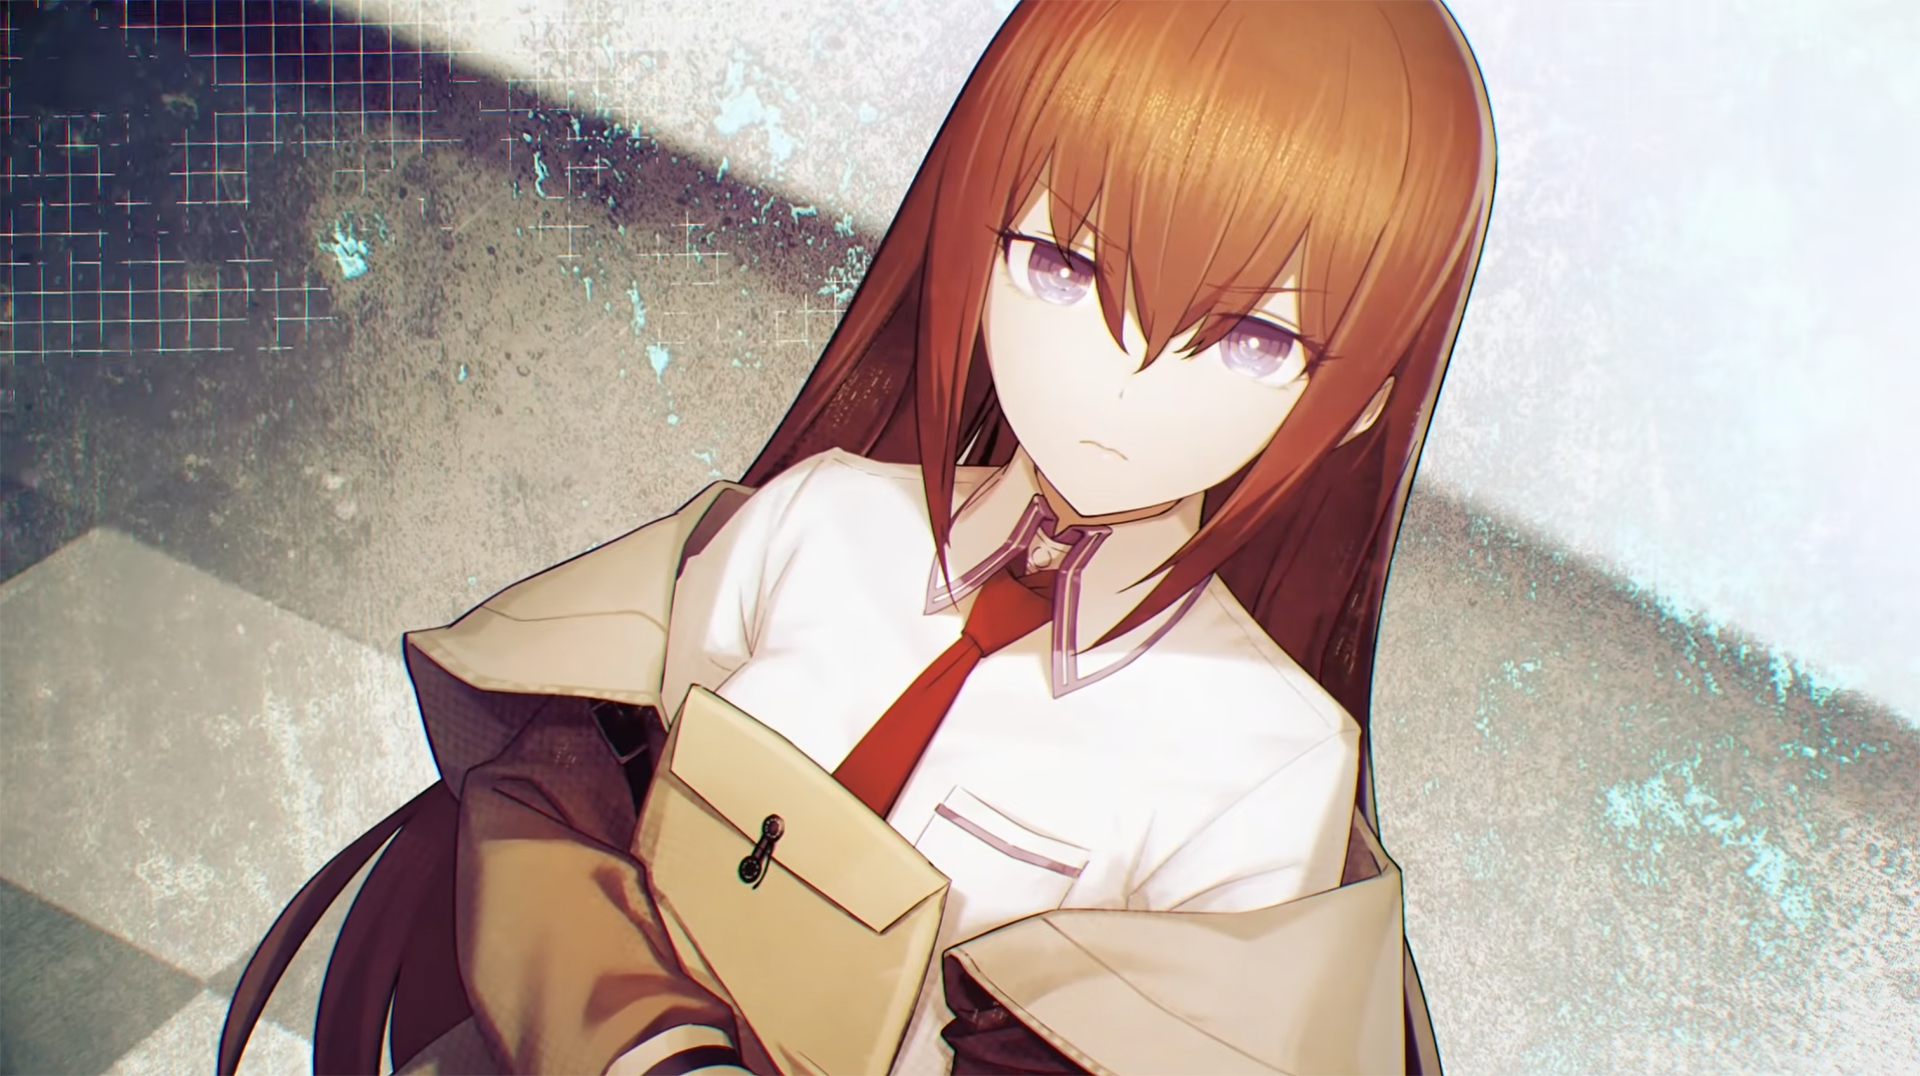
\includegraphics[width=0.98\textwidth]{graphics/kurisu_reboot.png}
            \end{center}
        \end{column}
        \begin{column}{0.45\textwidth}
            \begin{block}{Field Notes}
                \small
                \begin{itemize}
                    \item Rarely seen without a document case tucked under one arm
                    \item That stare alone has ended more of Okabe's harebrained theories than any experiment has
                    \item Her lab coat functions less like a uniform and more like a security blanket
                \end{itemize}
            \end{block}
            \vspace{0.3cm}
            \begin{exampleblock}{Status}
                \centering \small Still the smartest person in the room.\\ Still 34 today. Still not amused.
            \end{exampleblock}
        \end{column}
    \end{columns}
\end{frame}

% --- Slide 7: Trivia / Fun Facts ---
\begin{frame}{Declassified Lab Trivia}
    \begin{itemize}
        \item Her given name ``Kurisu'' shares its reading with \textit{kuri} (chestnut), which fits given her chestnut-to-auburn hair
        \item Secretly, not so secretly, loves \textbf{pudding}, and gets defensive the moment anyone notices
        \item Surprisingly \textbf{afraid of cats}, a detail she would prefer stayed out of every lab report
        \item Voiced by Asami Imai in Japanese and Trina Nishimura in English
        \item Her storyline is widely considered the anime's ``true route,'' the one where both she and Mayuri make it out fine
        \item Won the 2014 AnimeBracket ``Best Girl'' contest with 6{,}620 votes, a result she would insist means nothing
    \end{itemize}
    \vspace{0.3cm}
    \begin{block}{Lab Directive}
        \centering \small For research purposes only. Do not attempt to verify the pudding fact by hiding some in the lab fridge.
    \end{block}
\end{frame}

% --- Slide 8: Closing / Birthday Message ---
{
\setbeamercolor{background canvas}{bg=LabDeepBlue}
\begin{frame}
    \begin{center}
        \vspace{0.3cm}
        
\includegraphics[height=2.1cm]{graphics/fg.png}\\[10pt]
        {\usebeamercolor[fg]{title}\Huge\bfseries\color{white} Happy Birthday, Christina!}\\[10pt]
        {\color{white!85!black}\large Lab Member 004, may your world line always lead somewhere good.}

        \vspace{0.5cm}
        \begin{block}{}
            \begin{center}
            {\color{black}\itshape ``I-It's not like I wanted a whole presentation made about me or anything. \\
            But fine. Thank you. Don't let it go to your head.''}
            \end{center}
        \end{block}

        \vspace{0.3cm}
        {\small\color{white!70!black} Filed by the Future Gadget Lab, without her consent, but with her permission to be quoted, probably}
    \end{center}
\end{frame}
}

\end{document}
